\chapter{Πειραματικός Έλεγχος Συστήματος} \label{ch:demo}
\markboth{Πειραματικός Έλεγχος Συστήματος}{}

Στην ενότητα αυτή παρουσιάζονται μερικά αποτελέσματα που αφορούν τον πειραματικό έλεγχο ορθής λειτουργίας του συστήματος πλοήγησης που προτάθηκε. Αρχικά, πρέπει να το τονιστεί το γεγονός πως οι χρονικοί περιορισμοί της διπλωματικής εργασίας δεν επέτρεψαν την διενέργεια ενός επίσημου τεστ χρηστικότητας σε πραγματικούς χρήστες με προβλήματα όρασης. Παρόλα αυτά έγινε μια προσπάθεια ελέγχου κάθε ξεχωριστού τμήματος της διπλωματικής πριν την ενσωμάτωσή του στο υπόλοιπο σύστημα, όπως επίσης και συνολικός έλεγχος ολόκληρου του συστήματος. Για την πληρέστερη περιγραφή έγινε καταγραφή ενός βίντεο επίδειξης (demo), στο οποίο παρουσιάζονται οι δυνατότητες του υλοποιηθέντος συστήματος πλοήγησης. Το βίντεο μπορείτε να το βρείτε στο ακόλουθο λινκ \url{https://youtu.be/2TiHW27NSLQ}.

\section{Απόδοση αλγορίθμων}
Κάθε αλγόριθμος που παρουσιάστηκε στην ενότητα της υλοποίησης δοκιμάζεται και ελέγχεται κατά πόσο λειτουργεί αποτελεσματικά και σύμφωνα με τις προδιαγραφές που ορίστηκαν. Είναι σημαντικό να τονίσουμε ότι, αν και στην αρχή το πρόγραμμα είχε πολύ χαμηλά fps (frames per second), μετά από κατάλληλες τροποποιήσεις στον κώδικα και στην λογική των αλγορίθμων η ταχύτητα κυμαίνεται στο εύρος 20-30fps, το οποίο είναι ένα πολύ καλό νούμερο για εφαρμογές πραγματικού χρόνου.

\subsection{Εντοπισμός διάβασης πεζών}
Ο αλγόριθμος εντοπισμού διαβάσεων λειτουργεί αρκετά αποτελεσματικά κάτω από φυσιολογικές συνθήκες φωτισμού και τα πάει αρκετά καλά ακόμα και σε πιο ακραίες συνθήκες, όπως βρεγμένος δρόμος ή αντανακλάσεις από τον ήλιο. Είναι γεγονός πως σε συνθήκες πολύ χαμηλού φωτισμού, όπως π.χ. όταν επικρατεί σκοτάδι, δεν μπορεί να λειτουργήσει αποδοτικά. Παρακάτω, παρατίθενται παραδείγματα διαβάσεων που αναγνωρίζονται από τον προτεινόμενο αλγόριθμο, καθώς και μερικές περιπτώσεις στις οποίες "εξαπατάται" από το οπτικό περιβάλλον, όπως για παράδειγμα στην ύπαρξη σκαλιών.
\begin{figure}[H]
    \centering
    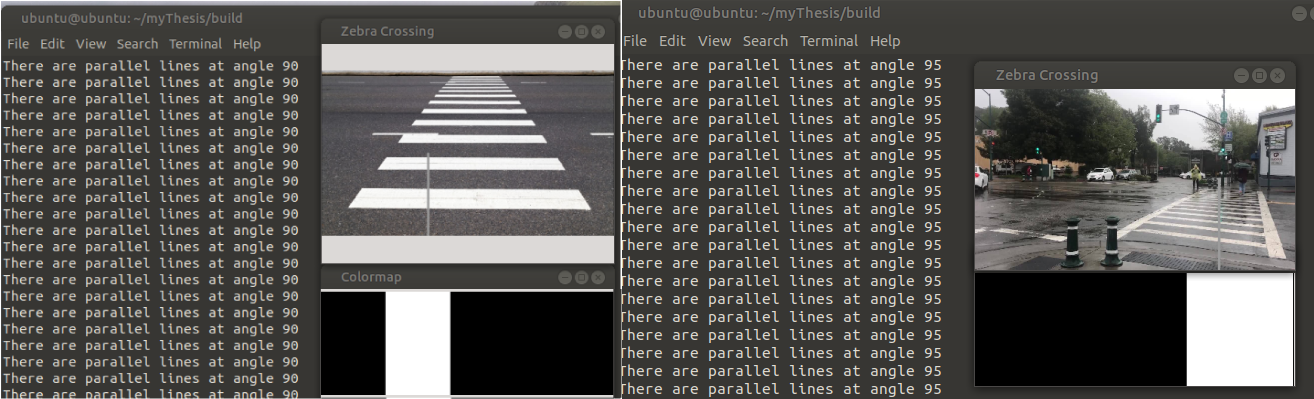
\includegraphics[width=\textwidth]{images/test_zebra1.png}
    \caption{Παράδειγμα εντοπισμού διάβασης πεζών. Η γκρίζα ευθεία γραμμή πάνω στη διάβαση, καθώς και η λευκή περιοχή κάτω από την διάβαση υποδηλώνουν το βέλτιστο μονοπάτι που πρέπει να ακολουθήσει ο χρήστης. Επίσης, το πρόγραμμα εμφανίζει και την κλίση των γραμμών της διάβασης σε μοίρες. Απλή διάβαση (αριστερά), βρεγμένη διάβαση (δεξιά).}
    \label{fig:test-zebra1}
\end{figure}
\begin{figure}[H]
    \centering
    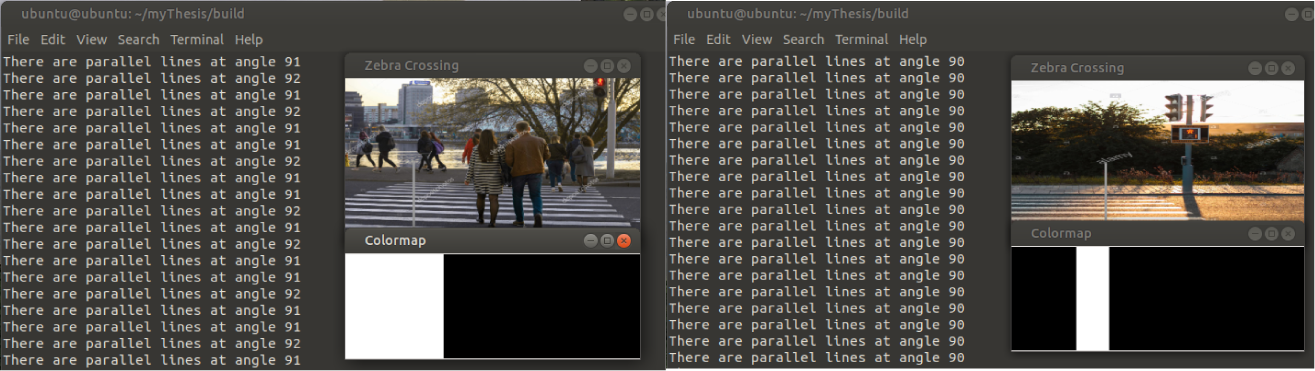
\includegraphics[width=\textwidth]{images/test_zebra3.png}
    \caption{Παράδειγμα εντοπισμού διάβασης πεζών με παρουσία εμποδίων (αριστερά) ή αντανάκλασης ηλιακού φωτός (δεξιά)}
    \label{fig:test-zebra3}
\end{figure}
\begin{figure}[H]
    \centering
    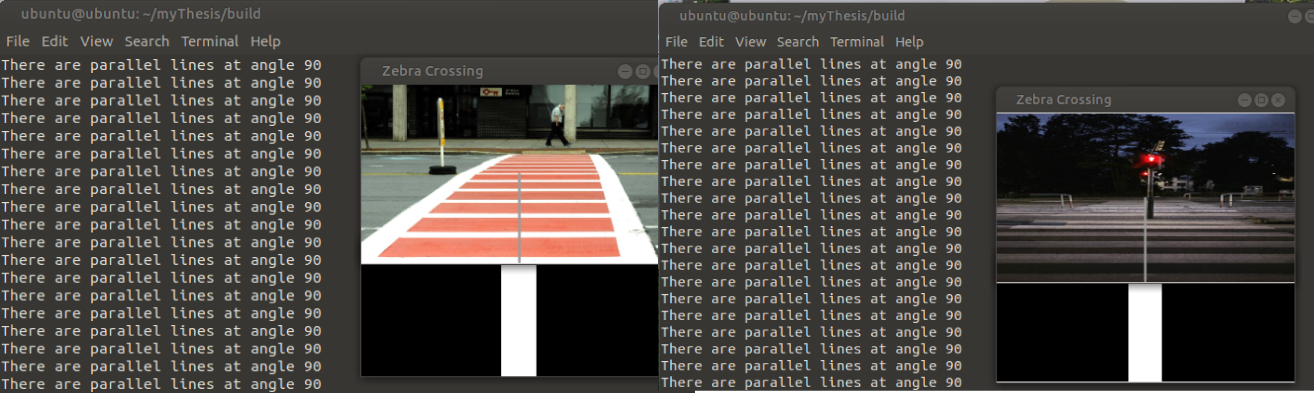
\includegraphics[width=\textwidth]{images/test_zebra2.png}
    \caption{Παράδειγμα εντοπισμού διάβασης πεζών άλλων χρωματικών αποχρώσεων (αριστερά) ή σε σκοτεινό περιβάλλον (δεξιά)}
    \label{fig:test-zebra2}
\end{figure}
\subsection{Αναγνώριση φωτεινού σηματοδότη}
Ο αλγόριθμος αναγνώρισης φωτεινού σηματοδότη λειτουργεί επαρκώς καλά κάτω από συγκεκριμένες συνθήκες. Η αποτελεσματικότητά του επηρεάζεται άμεσα από την ένταση της φωτεινότητας του φαναριού, την ανάλυση της κάμερας, την γωνία λήψης της φωτογραφίας και τις εξωτερικές συνθήκες περιβάλλοντος, π.χ. συννεφιά, βροχή κλπ. Ωστόσο, η χρήση του κάτω από συνηθισμένες συνθήκες δίνει ικανοποιητικά αποτελέσματα.
\begin{figure}[H]
    \centering
    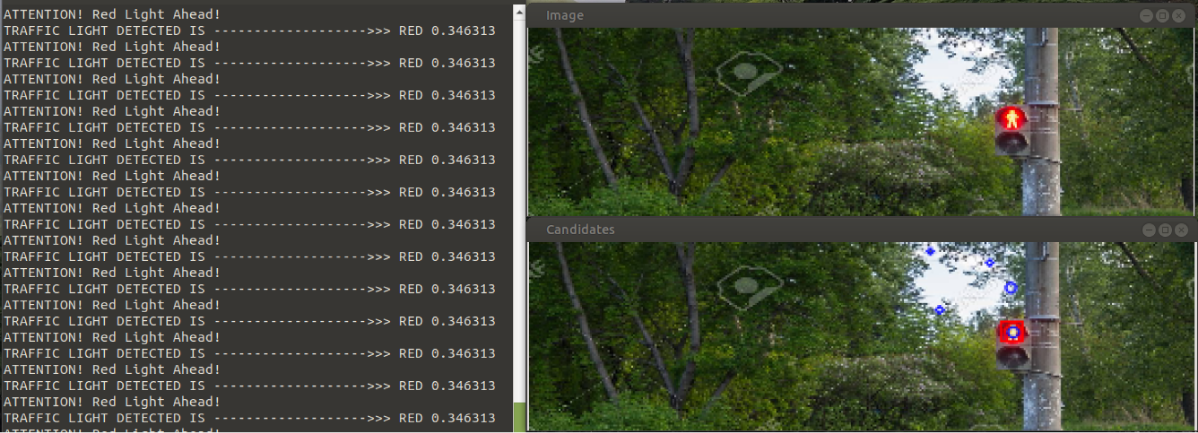
\includegraphics[width=0.9\textwidth]{images/test_light1.png}
    \caption{Παράδειγμα αναγνώρισης κόκκινου φωτεινού σηματοδότη (κόκκινο περίγραμμα γύρω από το φανάρι). Οι μπλε κύκλοι υποδηλώνουν πιθανές περιοχές με φωτεινό σηματοδότη που εντοπίστηκαν από τον αλγόριθμο, αλλά δεν πέρασαν τη φάση της επικύρωσης (validation). Τα νούμερα που φαίνονται αριστερά στην κονσόλα είναι η τιμή του μέτρου σύγκρισης κατά την εφαρμογή του template matching.}
    \label{fig:test-light1}
\end{figure}
\begin{figure}[H]
    \centering
    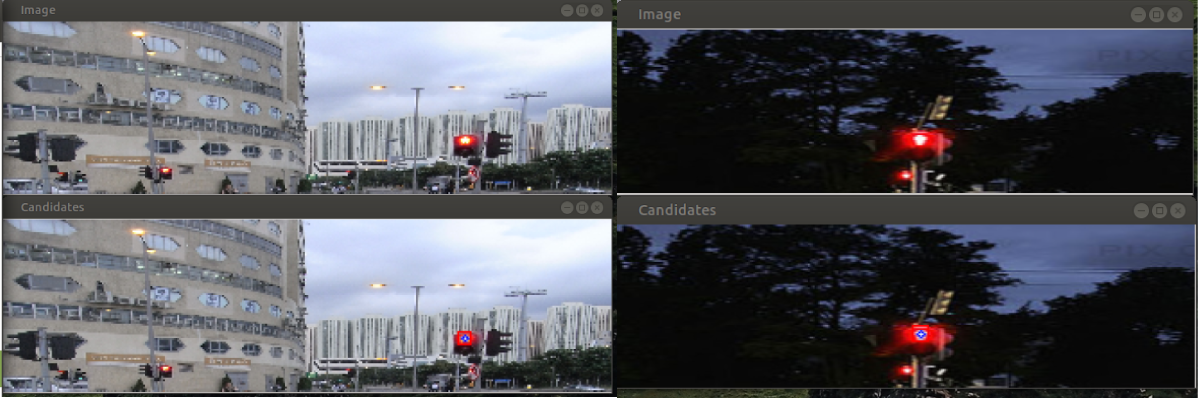
\includegraphics[width=0.9\textwidth]{images/test_light2.png}
    \caption{Παραδείγματα αναγνώρισης κόκκινου φωτεινού σηματοδότη (κόκκινο περίγραμμα γύρω από το φανάρι).}
    \label{fig:test-light2}
\end{figure}
\begin{figure}[H]
    \centering
    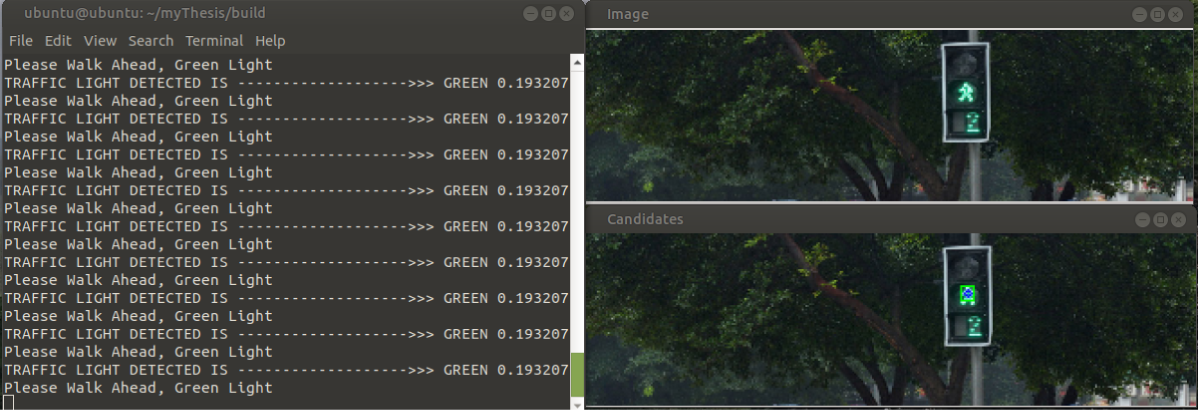
\includegraphics[width=0.9\textwidth]{images/test_light3.png}
    \caption{Παράδειγμα αναγνώρισης πράσινου φωτεινού σηματοδότη (πράσινο περίγραμμα γύρω από το φανάρι).}
    \label{fig:test-light3}
\end{figure}
\begin{figure}[H]
    \centering
    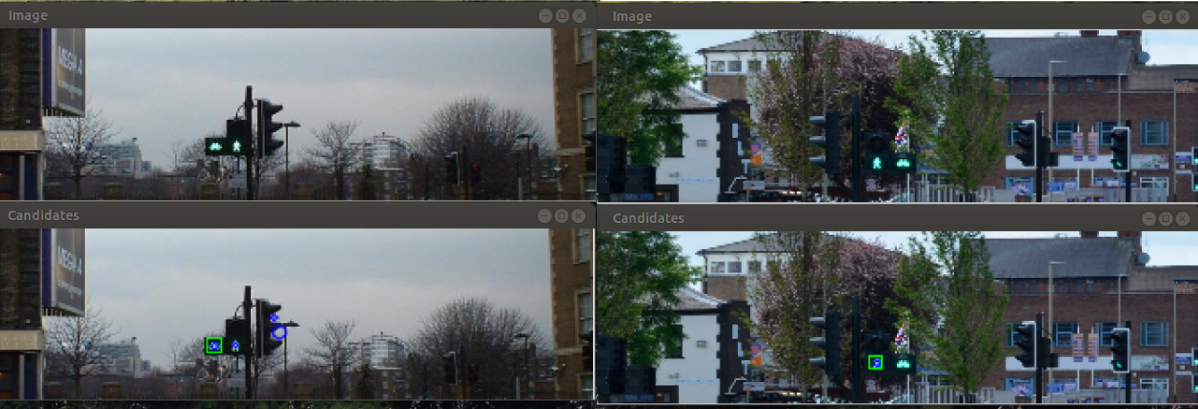
\includegraphics[width=0.9\textwidth]{images/test_light4.png}
    \caption{Παραδείγματα αναγνώρισης πράσινου φωτεινού σηματοδότη (πράσινο περίγραμμα γύρω από το φανάρι). Οι μπλε κύκλοι υποδηλώνουν πιθανές περιοχές με φωτεινό σηματοδότη που εντοπίστηκαν από τον αλγόριθμο, αλλά δεν πέρασαν τη φάση της επικύρωσης (validation). Τα νούμερα που φαίνονται αριστερά στην κονσόλα είναι η τιμή του μέτρου σύγκρισης κατά την εφαρμογή του template matching.}
    \label{fig:test-light4}
\end{figure}

\subsection{Αποφυγή εμποδίων}
Ο αλγόριθμος αποφυγής εμποδίων είναι ο πιο απλός αλγόριθμος του συστήματος. Λειτουργεί αποτελεσματικά στις περισσότερες περιπτώσεις, ενώ είναι ιδιαίτερα ανθεκτικός σε συνθήκες φωτισμού και εξωτερικού περιβάλλοντος.

\begin{figure}[H]
    \centering
    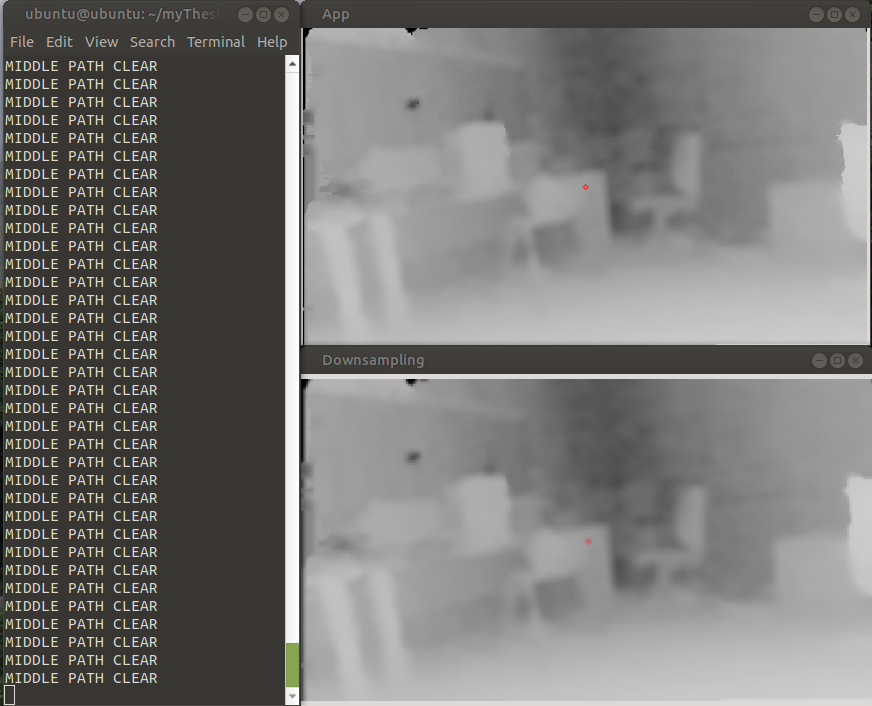
\includegraphics[width=0.8\textwidth]{images/test_depth_clear.png}
    \caption{Παράδειγμα εντοπισμού εμποδίων. Η κεντρική περιοχή της εικόνας βάθους είναι κενή, άρα το σύστημα ειδοποιεί τον χρήστη να προχωρήσει ελεύθερα.}
    \label{fig:test-depth-clear}
\end{figure}
\begin{figure}[H]
    \centering
    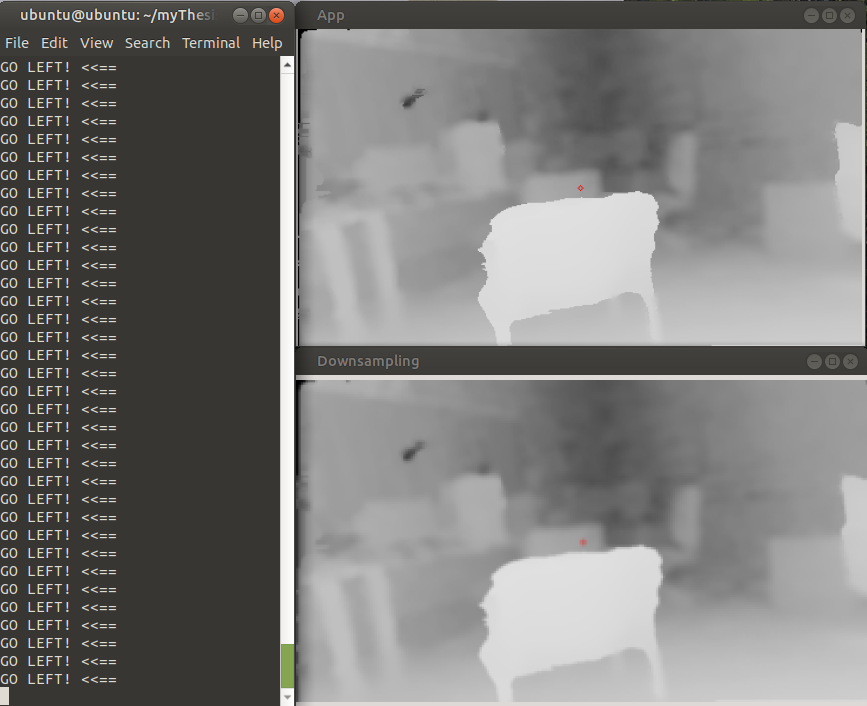
\includegraphics[width=0.7\textwidth]{images/test_depth_left.png}
    \caption{Παράδειγμα εντοπισμού εμποδίων. Η κεντρική περιοχή της εικόνας βάθους είναι κατειλημμένη από εμπόδιο, άρα το σύστημα ειδοποιεί τον χρήστη να μετακινηθεί αριστερά στον κενό χώρο.}
    \label{fig:test-depth-left}
\end{figure}
\begin{figure}[H]
    \centering
    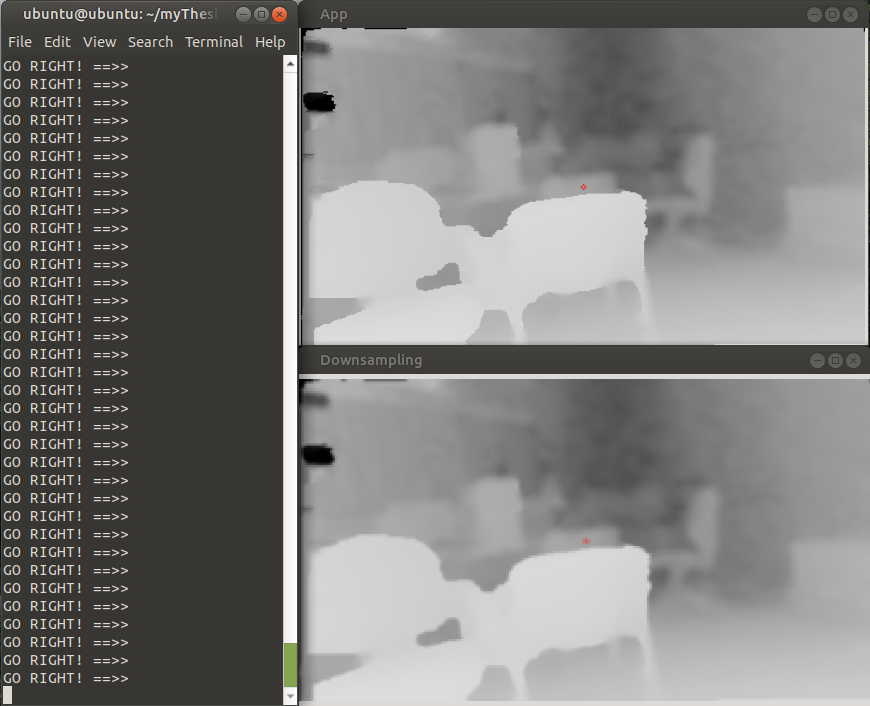
\includegraphics[width=0.7\textwidth]{images/test_depth_right.png}
    \caption{Παράδειγμα εντοπισμού εμποδίων. Τόσο η κεντρική, όσο και η αριστερή περιοχή της εικόνας βάθους είναι κατειλημμένες από εμπόδια, άρα το σύστημα ειδοποιεί τον χρήστη να μετακινηθεί δεξιά στον κενό χώρο.}
    \label{fig:test-depth-right}
\end{figure}

\section{Απτική ανάδραση}
Η χρήση απτικής ανάδρασης για την ειδοποίηση του χρήστη είναι από τα πιο δυνατά χαρακτηριστικά του συστήματος. Παρέχει διακριτικότητα και δίνει στον χρήστη την άνεση να μετακινείται στον χώρο χωρίς να απαιτείται η χρήση κάποιου ακουστικού. Τα μοτίβα δονήσεων (haptic icons), όπως παρουσιάστηκαν στην ενότητα 3.4.4, είναι ευδιάκριτα μεταξύ τους χάρη στον περιορισμένο αριθμό τους και στην χρήση κατάλληλων συνδυασμών παύσης, δόνησης και έντασης σε κάθε ξεχωριστό μοτίβο. Το γεγονός αυτό καθιστά την εκμάθησή τους εύκολη και γρήγορη, ενώ αναδεικνύεται η καταλληλότητά τους για ένα σύστημα πλοήγησης για άτομα με προβλήματα όρασης.

\section{Τελική διάταξη}
Η τελική διάταξη του πειραματικού συστήματος περιλαμβάνει την ενσωμάτωση όλου του εξοπλισμού (Raspberry Pi 4, Camera, Powerbank) σε ένα τσαντάκι μέσης, που λειτουργεί ως μέσο στήριξης, για την εύκολη και άνετη χρήση του από το άτομο με προβλήματα όρασης. Στο σχήμα \ref{fig:final-version} φαίνεται η τελική μορφή του συστήματος πάνω στον χρήστη. Ο χρήστης, πέρα από το τσαντάκι μέσης με τον εξοπλισμό, κρατάει και το smartphone από το οποίο δέχεται ανάδραση.

\begin{figure}[H]
    \centering
    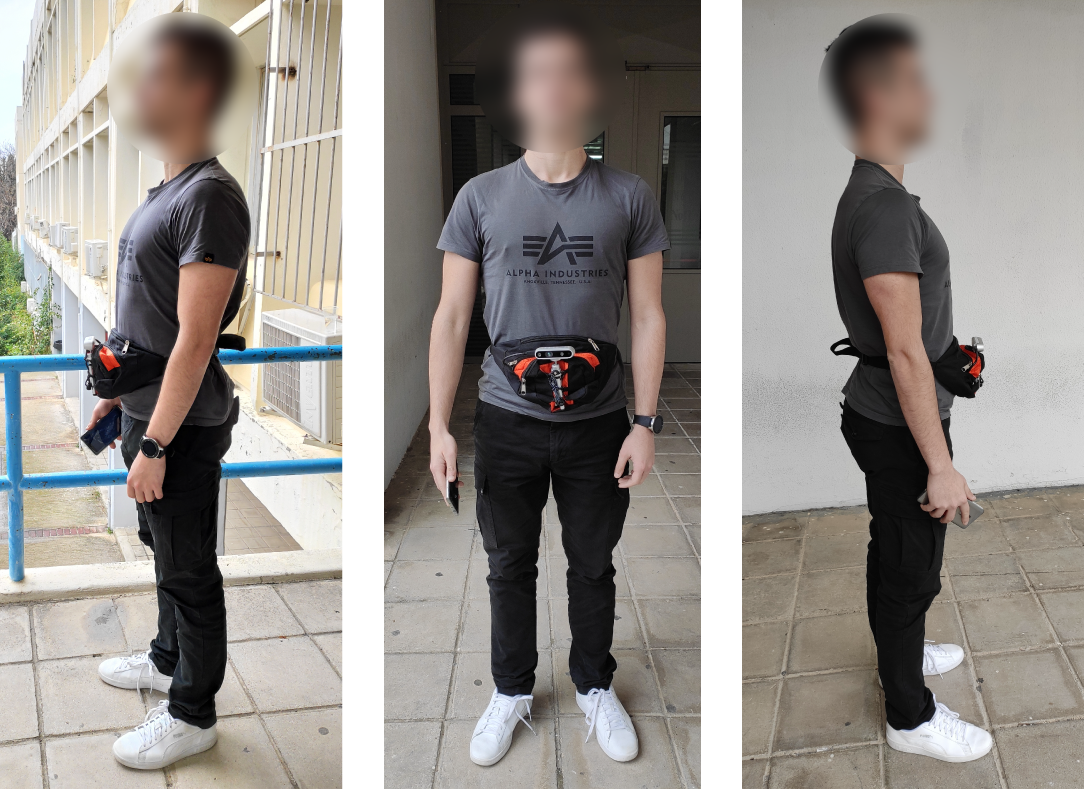
\includegraphics[width=\textwidth]{images/final-version.png}
    \caption{Τελική διάταξη προτεινόμενου συστήματος}
    \label{fig:final-version}
\end{figure}